\documentclass[level=2]{kidscode}
% Let lines with long code words stretch a little instead of running into the margin.
\setlength{\emergencystretch}{3em}

% A small helper for question headings inside the papers.
\newcounter{kcq}
\newcommand{\question}[2]{\stepcounter{kcq}\par\needspace{5\baselineskip}\medskip
  \noindent{\large\bfseries Question \arabic{kcq}}\hfill{\small\bfseries #1}\par\nopagebreak
  \noindent #2\par}
% "I can" rubric row: four checkboxes.
\newcommand{\icanrow}[1]{#1 & $\square$ & $\square$ & $\square$ & $\square$ \\ \midrule}
\newenvironment{icanrubric}{\par\noindent\renewcommand{\arraystretch}{1.35}%
  \tabularx{\linewidth}{@{}X*{4}{>{\centering\arraybackslash}p{1.65cm}}@{}}
  \toprule
  \textbf{I can\ldots} & \textbf{Just starting} & \textbf{Getting there} & \textbf{Got it} & \textbf{Expert} \\ \midrule}
  {\endtabularx\par}

\begin{document}
\kctitle{Assessments}{Placement quiz, mid-level checkpoint and exit assessment}

\begin{tip}[For the teacher]
Print one paper per child when you need it: the \textbf{placement quiz} at the start of week 1,
the \textbf{checkpoint} in week 6 and the \textbf{exit assessment} in week 12. Children work alone,
with pencil and paper, no computer. You may read any question aloud. Answers, scoring guides and
the placement decision guide are in the Answer Key (section \enquote{Assessments}).
\end{tip}

\begin{tip}[For students]
These papers help your teacher choose the right challenges for you. They are not about passing or
failing. If you do not know an answer, write what you think or draw a question mark: that is
useful too!
\end{tip}

%% =====================================================================
\kcpart{Quiz}{Placement Quiz}{Before Level 2 \textperiodcentered{} 15 minutes \textperiodcentered{} Show me what you remember from Level 1 Python.}
\setcounter{kcq}{0}
\namedateline

\question{2 points}{What does this program print? Write every line.}
\begin{pycode}
for i in range(3):
    print("Hip")
print("Hooray!")
\end{pycode}
\answerlines{3}

\question{1 point}{What does this program print?}
\begin{pycode}
coins = 5
coins = coins + 3
print(coins)
\end{pycode}
\answerlines{1}

\question{1 point}{What does this turtle draw? Circle one.}
\begin{pycode}
import turtle
t = turtle.Turtle()
for i in range(4):
    t.forward(100)
    t.left(90)
turtle.done()
\end{pycode}
\begin{center}
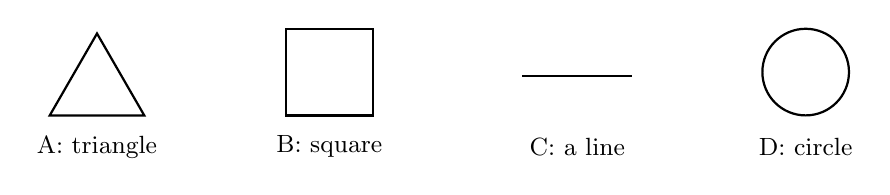
\begin{tikzpicture}[every node/.style={font=\small}]
  \draw[thick] (0,0) -- (1.2,0) -- (0.6,1.04) -- cycle; \node at (0.6,-0.4) {A: triangle};
  \draw[thick] (3,0) rectangle (4.1,1.1);                \node at (3.55,-0.4) {B: square};
  \draw[thick] (6,0.5) -- (7.4,0.5);                     \node at (6.7,-0.4) {C: a line};
  \draw[thick] (9.6,0.55) circle (0.55);                 \node at (9.6,-0.4) {D: circle};
\end{tikzpicture}
\end{center}

\question{2 points}{The player types a number. What does the program print\ldots}
\begin{pycode}
n = int(input("Pick a number: "))
if n > 10:
    print("Big")
elif n > 5:
    print("Medium")
else:
    print("Small")
\end{pycode}
\noindent a) \ldots if the player types \texttt{7}? \rule{4cm}{0.4pt}\par\noindent
b) \ldots if the player types \texttt{10}? \rule{4cm}{0.4pt}

\question{2 points}{This program has \textbf{two} bugs. Circle them and write the fixed lines.}
\begin{pycode}
import turtle
t = turtle.Turtle()
for i in range(3)
    t.forwad(80)
    t.left(120)
turtle.done()
\end{pycode}
\answerlines{2}

\question{1 point}{\texttt{random.randint(1, 6)} picks a random number. Which numbers can it give?}
\answerlines{1}

\question{2 points}{Read the program, then answer.}
\begin{pycode}
import turtle
t = turtle.Turtle()

def star(size):
    for i in range(5):
        t.forward(size)
        t.right(144)

star(50)
star(100)
turtle.done()
\end{pycode}
\noindent a) How many stars are drawn? \rule{2cm}{0.4pt}\par\noindent
b) Which star is bigger, the first or the second? \rule{3cm}{0.4pt}

\question{3 points}{Write a program that prints \texttt{Go team!} four times, using a \texttt{for} loop.}
\answerspace{3cm}

\question{Bonus, 1 point}{Change your program so it prints the numbers 1, 2, 3, 4 before each \texttt{Go team!}}
\answerspace{2cm}

\subsection{How did that feel? (not scored)}
\begin{icanrubric}
\icanrow{I can read a short Python program and say what it prints.}
\icanrow{I can use a \texttt{for} loop with \texttt{range}.}
\icanrow{I can use \texttt{if}, \texttt{elif} and \texttt{else}.}
\icanrow{I can find and fix a typo or a missing colon.}
\icanrow{I can write a function with \texttt{def}.}
\end{icanrubric}

%% =====================================================================
\kcpart{Week 6}{Mid-Level Checkpoint}{About 15 minutes \textperiodcentered{} Types, functions, lists, while loops and dictionaries.}
\setcounter{kcq}{0}
\namedateline

\question{2 points}{Draw a line from each value to its type.}
\begin{center}
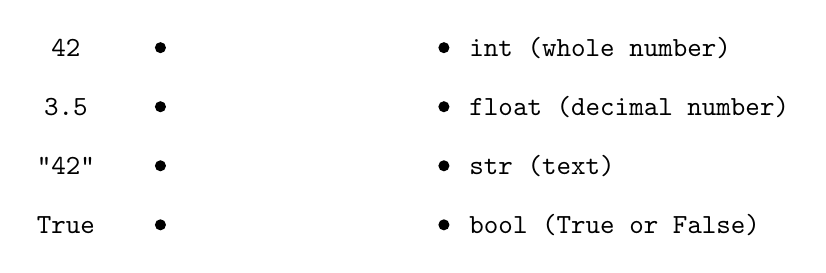
\begin{tikzpicture}[every node/.style={font=\ttfamily}, node distance=0.75cm]
  \node (a) at (0,0)    {42};
  \node (b) at (0,-0.75) {3.5};
  \node (c) at (0,-1.5) {"42"};
  \node (d) at (0,-2.25) {True};
  \node[anchor=west] at (5,0)    {int   (whole number)};
  \node[anchor=west] at (5,-0.75) {float (decimal number)};
  \node[anchor=west] at (5,-1.5) {str   (text)};
  \node[anchor=west] at (5,-2.25) {bool  (True or False)};
  \foreach \y in {0,-0.75,-1.5,-2.25} {\fill (1.2,\y) circle (2pt); \fill (4.8,\y) circle (2pt);}
\end{tikzpicture}
\end{center}

\question{1 point}{What does this print?}
\begin{pycode}
hero = "Kai"
stars = 3
print(f"{hero} has {stars * 2} stars")
\end{pycode}
\answerlines{1}

\question{2 points}{What does this print?}
\begin{pycode}
def double(n):
    return n * 2

x = double(4) + 1
print(x)
print(double(double(1)))
\end{pycode}
\answerlines{2}

\question{2 points}{What does this print?}
\begin{pycode}
colors = ["orange", "sky blue", "green"]
colors.append("purple")
print(len(colors))
print(colors[1])
\end{pycode}
\answerlines{2}

\question{2 points}{Fill in the trace table, then write what the program prints.
Write the value of \texttt{count} each time it changes.}
\begin{pycode}
count = 1
while count < 50:
    count = count * 3
print(count)
\end{pycode}
\begin{center}
\renewcommand{\arraystretch}{1.4}
\begin{tabular}{|p{3cm}|p{1.5cm}|p{1.5cm}|p{1.5cm}|p{1.5cm}|p{1.5cm}|}
\hline
\textbf{value of count} & 1 & & & & \\ \hline
\end{tabular}
\end{center}
\noindent It prints: \rule{3cm}{0.4pt}

\question{1 point}{What does this print?}
\begin{pycode}
points = {"star": 5, "moon": 10}
points["comet"] = 20
print(points["moon"] + points["comet"])
\end{pycode}
\answerlines{1}

\question{2 points}{Sam's program prints 20 and then crashes with this error. Find the bug and fix it.}
\begin{outputcode}
TypeError: unsupported operand type(s) for +: 'NoneType' and 'int'
\end{outputcode}
\begin{pycode}
def area(width, height):
    print(width * height)

bigger = area(4, 5) + 1
print(bigger)
\end{pycode}
\answerlines{2}

\question{1 point}{This crashes with \texttt{KeyError: 'Cat'}. Fix it.}
\begin{pycode}
pets = {"cat": 2, "dog": 1}
print(pets["Cat"])
\end{pycode}
\answerlines{1}

\question{3 points}{Write a function \texttt{count\_stars(items)} that \textbf{returns} how many times
\texttt{"star"} is in the list \texttt{items}. For example,
\texttt{count\_stars(["star", "moon", "star"])} should return \texttt{2}.}
\answerspace{4.2cm}

\question{2 points}{You get a long red error message (a traceback). Where do you start reading, and why?}
\answerlines{2}

\subsection{My checkpoint rubric}
Check one box in each row. Be honest: this helps us plan the next weeks.
\begin{icanrubric}
\icanrow{I can tell int, float, str and bool apart and build messages with f-strings.}
\icanrow{I can write a function that uses \texttt{return}.}
\icanrow{I can make a list, add to it and get items by index.}
\icanrow{I can write a \texttt{while} loop that stops.}
\icanrow{I can store and look up values in a dictionary.}
\icanrow{I can read a traceback and use a debugging strategy.}
\end{icanrubric}

%% =====================================================================
\kcpart{Week 12}{Exit Assessment}{About 20 minutes \textperiodcentered{} Files, tests and event-driven programs: read, predict, fix, write and explain.}
\setcounter{kcq}{0}
\namedateline

\question{2 points}{What does this print?}
\begin{pycode}
with open("pets.txt", "w") as file:
    file.write("cat\n")
with open("pets.txt", "a") as file:
    file.write("fish\n")
with open("pets.txt") as file:
    lines = file.read().split()
print(len(lines), lines[0])
\end{pycode}
\answerlines{1}

\question{1 point}{In the program above, what would be in \texttt{pets.txt} if the second
\texttt{open} used \texttt{"w"} instead of \texttt{"a"}? Why?}
\answerlines{2}

\question{2 points}{The first time Priya runs her game, this line crashes with
\texttt{FileNotFoundError}. Why? Rewrite it so the game starts with an empty list instead.}
\begin{pycode}
with open("scores.txt") as file:
    scores = file.read().split()
\end{pycode}
\answerspace{3.2cm}

\question{3 points}{Here is a function and one test.}
\begin{pycode}
def clamp(value, low, high):
    if value < low:
        return low
    if value > high:
        return high
    return value

def test_clamp_normal():
    assert clamp(5, 0, 10) == 5
\end{pycode}
\noindent a) Will this test pass or fail? \rule{3cm}{0.4pt}\\[4pt]
b) Leo writes \py|assert clamp(-3, 0, 10) == -3|. It fails. Is the bug in the function or in the test? Explain.
\answerlines{2}
\noindent c) Write one \textbf{edge case} test for \texttt{clamp}.
\answerlines{2}

\question{2 points}{Mei wants the space key to make the player jump, but the player jumps once at
the start and then never again. Find the bug and fix the line.}
\begin{pycode}
def jump():
    player.sety(player.ycor() + 50)

screen.onkey(jump(), "space")
screen.listen()
\end{pycode}
\answerlines{1}
\noindent What does \texttt{screen.listen()} do? \answerlines{1}

\question{2 points}{A game loop uses \texttt{ontimer}. The program starts it by calling \texttt{tick()} one time.
After that, only \texttt{ontimer} calls it. (100 means 100 milliseconds.)}
\begin{pycode}
game = {"ticks": 0}

def tick():
    game["ticks"] = game["ticks"] + 1
    if game["ticks"] < 5:
        screen.ontimer(tick, 100)
\end{pycode}
\noindent a) How many times does \texttt{tick} run in total? \rule{2cm}{0.4pt}\par\noindent
b) What is \texttt{game["ticks"]} at the end? \rule{2cm}{0.4pt}

\question{1 point}{In a catching game, what does this line check? Explain in your own words.}
\begin{pycode}
if basket.distance(star) < 30:
\end{pycode}
\answerlines{2}

\question{4 points}{Write a function \texttt{best\_score(scores)} that \textbf{returns} the biggest
number in the list \texttt{scores}, or \texttt{0} if the list is empty. Then write one test for it.}
\answerspace{5.5cm}

\question{3 points}{Explain one function from \textbf{your} final project: what goes in
(parameters), what comes out (return value), and how you tested it.}
\answerlines{4}

\subsection{My Level 2 rubric}
\begin{icanrubric}
\icanrow{I can save data to a file and load it again.}
\icanrow{I can write pytest tests for normal and edge cases.}
\icanrow{I can make a program react to keys and timers.}
\icanrow{I can read code and predict what it does.}
\icanrow{I can find and fix bugs with a strategy.}
\icanrow{I can explain how my code works and why I made it that way.}
\end{icanrubric}

\begin{reflection}[Looking back]
What are you proudest of in Level 2? What do you want to learn next?
\answerlines{3}
\end{reflection}

\end{document}
